\documentclass{article}
\usepackage{amsmath}
\usepackage{amssymb}
\usepackage{amsthm}
\usepackage{geometry}
\usepackage{tikz}
\usepackage{tikz-cd}
\usepackage{listings}
\usepackage{booktabs}
\usepackage{microtype}
\usepackage{placeins}
\usepackage[hyphens]{url}
\usepackage{float}
\geometry{margin=1in}
\theoremstyle{plain}
\newtheorem{theorem}{Theorem}[section]
\newtheorem{proposition}[theorem]{Proposition}
\theoremstyle{definition}
\newtheorem{definition}[theorem]{Definition}
\title{From RSVP Fields to Mechanistic Self-Aware Machines}
\author{Flyxion}
\date{September 05, 2025}

\begin{document}

\maketitle

\begin{abstract}
This paper aims to unify field-theoretic physics with cognitive modeling by integrating the Relativistic Scalar-Vector Plenum (RSVP) framework with Bennett’s mechanistic model of AI self-awareness. Using category theory, we define $\mathbf{Mech}$ and $\mathbf{RSVP}$, construct a functor $F: \mathbf{Mech} \to \mathbf{RSVP}$, and prove properties including non-diverging Gr\"uneisen parameters via q-entropy and sheaf cohomology, incorporating error-correction inspired by magnetic proofreading self-assembly. Results include rigorous categorical constructions, functoriality proofs, and computational recipes, with self-awareness modeled as a homotopy fixed point. Implications suggest a unified framework for physics, cognition, and self-assembly, with testable predictions for AI and physical systems.
\end{abstract}

\section{Introduction}

\subsection{Prerequisites}
Readers should be familiar with category theory (objects, morphisms, functors, natural transformations \cite{Awodey2010,Lawvere2009}), differential geometry (smooth manifolds, tangent bundles \cite{Kock2004}), and sheaf theory (presheaves, gluing conditions \cite{MacLane1992,Bredon1997}). Knowledge of statistical physics (entropy, critical phenomena \cite{Tsallis1988}) and causal inference (structural causal models \cite{Pearl2009}) is assumed.

\subsection{Motivation and Overview}
The Relativistic Scalar-Vector Plenum (RSVP) theory models physical systems as scalar ($\Phi$), vector ($\mathcal{v}$), and entropy ($\mathcal{S}_q$) fields over a fibered category, addressing critical phenomena without divergences using q-entropy and sheaf cohomology \cite{Soares2024,Tsallis1988,Soares2023prb,Soares2023physica}. Bennett’s mechanistic model posits that self-awareness arises from causal inference and intent attribution, implemented computationally \cite{Bennett2025}. Magnetic proofreading self-assembly demonstrates local error correction to achieve high-fidelity structures, offering a physical analogy to RSVP entropy control \cite{Liang2025}. This paper constructs a functor $F: \mathbf{Mech} \to \mathbf{RSVP}$, mapping mechanistic operations to field dynamics, and integrates proofreading mechanisms to stabilize entropy.

This work unifies thermodynamic criticality, cognitive modeling, and physical self-assembly. The exposition proceeds with preliminaries, category definitions, functorial mappings, hardware-type mappings, computational implementation, worked examples, and philosophical interpretations, concluding with testable predictions. TikZ diagrams illustrate key concepts.

\section{Mathematical Preliminaries}

\subsection{Category Theory}
A category $\mathcal{C}$ consists of objects $\text{Ob}(\mathcal{C})$, morphisms $\text{Hom}_{\mathcal{C}}(A, B)$, associative composition $\circ$, and identities $\text{id}_A$ \cite{Awodey2010,Lawvere2009}. A functor $F: \mathcal{C} \to \mathcal{D}$ preserves composition and identities. A natural transformation $\eta: F \Rightarrow G$ assigns morphisms $\eta_A: F(A) \to G(A)$ such that $G(f) \circ \eta_A = \eta_B \circ F(f)$. An adjunction $F \dashv G$ involves unit $\eta$ and counit $\epsilon$ satisfying triangle identities \cite{Spivak2014}.

\subsection{Sheaf Theory}
A sheaf $\mathcal{F}$ on a topological space $X$ assigns data $\mathcal{F}(U)$ to open sets $U \subseteq X$, with restriction maps and gluing: for cover $\{U_i\}$, compatible sections $\{s_i \in \mathcal{F}(U_i)\}$ glue uniquely \cite{MacLane1992,Bredon1997}. Cohomology $\check{H}^n(X, \mathcal{F})$ measures gluing obstructions.

\subsection{Entropy and Criticality}
Boltzmann-Gibbs entropy $S = -k \sum p_i \log p_i$ fails at critical points. Tsallis q-entropy $S_q = k \frac{1 - \sum p_i^q}{q-1}$ restores extensivity \cite{Tsallis1988}. The Gr\"uneisen parameter $\Gamma = \frac{\alpha}{C_p}$ quantifies anharmonicity, non-diverging with q-entropy \cite{Soares2023prb,Soares2024}.

\subsection{Mechanistic AI and Self-Assembly}
Structural causal models (SCMs) define variables and equations for inference \cite{Pearl2009}. Self-awareness involves intent attribution and self-modeling \cite{Bennett2025,Goguen1992}. Magnetic proofreading self-assembly uses external fields to stabilize correct configurations, analogous to entropy control \cite{Liang2025}.

\section{RSVP Theory Formalism}

\subsection{Prerequisites}
Assume a smooth manifold $\mathcal{M}$ with tangent bundle $T\mathcal{M}$. Sheaves are on the site of open sets with Zariski topology, valued in $\mathbf{Ab}$ (abelian groups). Fields satisfy PDEs derived from action functionals \cite{Kock2004}.

\begin{definition}
Objects: Triples $(\Phi, \mathcal{v}, \mathcal{S}_q)$ where:
- $\Phi \in C^\infty(\mathcal{M}, \mathbb{R})$ is a scalar field (e.g., $\Phi(x) = x^2$ for a quadratic potential).
- $\mathcal{v} \in \Gamma(T\mathcal{M})$ is a vector field (e.g., $\mathcal{v} = \partial_x$ on $\mathbb{R}$).
- $\mathcal{S}_q$ is a sheaf of entropies valued in $\mathbb{R}$, satisfying gluing \cite{MacLane1992}.
Morphisms: $f: (\Phi, \mathcal{v}, \mathcal{S}_q) \to (\Phi', \mathcal{v}', \mathcal{S}_q')$ as triples $(f_\Phi, f_\mathcal{v}, f_{\mathcal{S}_q})$, with $f_\Phi$ smooth (e.g., restriction $\Phi \to \Phi|_U$), $f_\mathcal{v}$ a bundle morphism, $f_{\mathcal{S}_q}$ a sheaf morphism. Composition: $(g \circ f) = (g_\Phi \circ f_\Phi, g_\mathcal{v} \circ f_\mathcal{v}, g_{\mathcal{S}_q} \circ f_{\mathcal{S}_q})$. Identities: $\text{id}_{(\Phi, \mathcal{v}, \mathcal{S}_q)} = (\text{id}_\Phi, \text{id}_\mathcal{v}, \text{id}_{\mathcal{S}_q})$. $\mathbf{RSVP}$ is enriched over $\mathbf{Vect}_\mathbb{R}$\footnote{Vector spaces over $\mathbb{R}$ for field values.} and $\mathbf{Top}$\footnote{Topological spaces for homotopy data.}, with monoidal product $\otimes$ as field concatenation.
\end{definition}

\begin{figure}[h!]
\centering
\begin{tikzcd}[scale=0.6, column sep=small, row sep=small, every node/.style={font=\small}, ampersand replacement=\&]
(\Phi, \mathcal{v}, \mathcal{S}_q) \arrow[r, "f"] \arrow[dr, "g \circ f"'] \& (\Phi', \mathcal{v}', \mathcal{S}_q') \arrow[d, "g"] \\
\& (\Phi'', \mathcal{v}'', \mathcal{S}_q'')
\end{tikzcd}
\caption{\raggedright Composition in $\mathbf{RSVP}$: Morphisms are triples preserving field structures, composed component-wise.}
\label{fig:rsvp_composition}
\end{figure}

\begin{proposition}
$\mathbf{RSVP}$ is a category.
\end{proposition}
\begin{proof}
Intuitively, $\mathbf{RSVP}$ structures field transformations to preserve physical constraints. \textbf{Associativity}: For morphisms $f: A \to B$, $g: B \to C$, $h: C \to D$, $(h \circ (g \circ f)) = (h_\Phi \circ (g_\Phi \circ f_\Phi), h_\mathcal{v} \circ (g_\mathcal{v} \circ f_\mathcal{v}), h_{\mathcal{S}_q} \circ (g_{\mathcal{S}_q} \circ f_{\mathcal{S}_q})) = ((h \circ g) \circ f)$, by associativity of smooth maps \cite{Kock2004}, bundle morphisms, and sheaf morphisms \cite{MacLane1992}. \textbf{Identities}: For object $A = (\Phi, \mathcal{v}, \mathcal{S}_q)$, $\text{id}_A \circ f = f \circ \text{id}_A = f$, as each component identity satisfies unit laws.
\end{proof}

The action is $\mathcal{A} = \int_{\mathcal{M}} \left( \frac{1}{2}(\nabla \Phi)^2 + \frac{1}{2}\|\mathcal{v}\|^2 + \lambda S_q \right) d\mu$, where $S_q(U) = k \frac{1 - \sum \rho(x)^q}{q-1}$ \cite{Tsallis1988}. The entropy flow $\Xi = \frac{\delta \mathcal{A}}{\delta g}$, Gr\"uneisen parameter $\Gamma_{RSVP} = - \frac{\partial \Xi / \partial T}{\partial^2 \mathcal{A} / \partial T^2}$. At $q = q^*$, sheaf gluing ensures finite curvature, $\text{Curv}(\mathcal{S}_{q^*}) < \infty$ \cite{Soares2024}.

\section{The Source Category: $\mathbf{Mech}$ (Mechanistic Models)}

\subsection{Prerequisites}
SCMs involve variables, structural equations, and interventions (do-calculus, \cite{Pearl2009}). The category $\mathbf{Prob}$ consists of probability spaces with stochastic kernels. $\mathbf{Mech}$ is enriched over $\mathbf{Prob}$ for probabilistic transitions \cite{Lawvere2009}.

\begin{definition}
Objects:
- Sensory data spaces $S$ (measurable spaces with $\sigma$-algebra, e.g., $\mathbb{R}^n$ for sensor readings).
- Actuator spaces $A$ (finite sets, e.g., \{move, stop\}).
- Internal state spaces $I$ (probability spaces for beliefs/preferences).
- Causal models $C$ (SCMs with structural equations \cite{Pearl2009}).
- Policies $\pi: I \to A$ (measurable maps).
- Models of other agents (theory-of-mind objects).
- Evaluative/objective modules mapping states to utilities/goals.
Morphisms:
- Observational: $S \to O$ (e.g., sensor reading to observation).
- Perceptual inference: $O \to I$ (e.g., observation to belief update).
- Action selection: $I \to A$.
- Causal update: $C \to C'$.
- Intervention: $do(a): C \to C_a$ (do-calculus \cite{Pearl2009}).
Composition: Sequential application of functions or kernels. Identities: No-op transformations (e.g., $\text{id}_S(s) = s$). $\mathbf{Mech}$ is enriched over $\mathbf{Prob}$\footnote{Probability spaces with stochastic kernels.} with monoidal product $\otimes$ (concatenation of sensor/action sets).
\end{definition}

\begin{figure}[h!]
\centering
\begin{tikzcd}[scale=0.6, column sep=small, row sep=small, every node/.style={font=\small}, ampersand replacement=\&]
S \arrow[r, "observe"] \arrow[dr, "infer \circ observe"'] \& O \arrow[d, "infer"] \\
\& I \arrow[r, "\pi"] \& A
\end{tikzcd}
\caption{\raggedright Composition in $\mathbf{Mech}$: Sequential operations from observation to inference to action.}
\label{fig:mech_composition}
\end{figure}

\begin{proposition}
$\mathbf{Mech}$ is a category.
\end{proposition}
\begin{proof}
Intuitively, $\mathbf{Mech}$ models sequential cognitive operations. \textbf{Associativity}: For morphisms $f: S \to O$, $g: O \to I$, $h: I \to A$, $(h \circ g) \circ f = h \circ (g \circ f)$, as function composition (or kernel composition) is associative \cite{Lawvere2009}. \textbf{Identities}: The identity $\text{id}_S: S \to S$ maps each observation to itself, satisfying $\text{id}_O \circ f = f \circ \text{id}_S = f$.
\end{proof}

\section{The Functor $F: \mathbf{Mech} \to \mathbf{RSVP}$}

\subsection{Object Mapping}
- Sensory data space $S \mapsto$ sensory-field section: restriction maps $\Phi|_{U_S}$, with sensory input as low-dimensional linear functionals on $\Phi$.
- Actuator space $A \mapsto$ actuator field action: local perturbations of $\Phi$ and $\mathcal{v}$ via pushforward; $A$ as compactly supported perturbation operator $\delta_A$.
- Internal state $I \mapsto$ persona-vector submanifold $\mathcal{M}_I$ parametrized by embeddings into compressed latent space (Yarncrawler projection). Beliefs as probability sheaf sections over $\mathcal{M}_I$.
- Causal model $C \mapsto$ response operator $\mathcal{R}_C$ on RSVP fields: maps interventions to updates via Green’s functions from RSVP PDE linearization.
- Policy $\pi: I \to A \mapsto$ composite morphism $\mathcal{M}_I \xrightarrow{\mathcal{P}_\pi} \text{Act} \xrightarrow{\delta} \text{Perturb}(\Phi, \mathcal{v})$, implemented via Yarncrawler projection and argmax (or softmax for stochastic policies).
- Semantic modules and persona-vector objects (embeddings or attractors).
- Derived objects: line-bundles of partition functions, sheaves of local distributions, homotopy colimit objects for merges \cite{MacLane1992,Awodey2010}.

\subsection{Morphism Mapping}
- Perceptual inference $\text{infer}: O \to I \mapsto F(\text{infer}): \Phi|_{U_S} \xrightarrow{\mathcal{E}} \mathcal{M}_I$.
- Action selection $\pi: I \to A \mapsto F(\pi): \mathcal{M}_I \xrightarrow{\mathcal{P}_\pi} \text{Act} \xrightarrow{\delta} \text{Perturb}(\Phi, \mathcal{v})$.
- Causal update $\text{update}: C \to C' \mapsto$ field-theoretic Bayesian update: modifies $\mathcal{R}_C$ via entropy sheaf annealing and reweighting (cohomology-class shift \cite{MacLane1992}).
- Field evolution operators: flow maps $\Phi \to \Phi'$.
- Projection or encoding morphisms: $\mathcal{E}: \Phi \to \mathcal{M}$.
- Coarse-graining, restriction, or extension maps between sheaf sections \cite{MacLane1992}.
- Homotopy colimit morphisms for merges: $\text{hocolim}$ \cite{Awodey2010}.
- Entropy transforms (Tsallis twist) as multiplicative automorphisms on partition-function line bundles \cite{Tsallis1988}.

\begin{figure}[h!]
\centering
\begin{tikzcd}[scale=0.6, column sep=small, row sep=small, every node/.style={font=\small}, ampersand replacement=\&]
S \arrow[r, "F"] \arrow[d, "infer"] \& \Phi|_{U_S} \arrow[d, "\mathcal{E}"] \\
I \arrow[r, "F"] \& \mathcal{M}_I \arrow[r, "\mathcal{P}_\pi \circ \delta"] \& \text{Perturb}(\Phi, \mathcal{v})
\end{tikzcd}
\caption{\raggedright Functor $F: \mathbf{Mech} \to \mathbf{RSVP}$, mapping sensory spaces to field sections and inference to encoding maps.}
\label{fig:functor_mapping}
\end{figure}

\begin{theorem}
$F$ preserves identities and composition \cite{Spivak2014}.
\end{theorem}
\begin{proof}
Intuitively, $F$ maps mechanistic processes to field dynamics consistently. \textbf{Identities}: For $\text{id}_S: S \to S$, $F(\text{id}_S) = \text{id}_{\Phi|_{U_S}}$, as $\text{id}_{\Phi|_{U_S}}(x) = \Phi(x)$. Similarly for $A$, $I$, $C$, $\pi$. \textbf{Composition}: For $f: S \to O$, $g: O \to I$, $F(g \circ f) = \mathcal{E}_g \circ \mathcal{E}_f = \mathcal{E}_{g \circ f}$, as encoding maps compose smoothly. For action $\pi: I \to A$, $F(\pi) = \mathcal{P}_\pi \circ \delta$, and $F(h \circ \pi) = F(h) \circ F(\pi)$ by composition of projections and perturbations.
\end{proof}

\begin{theorem}
$\text{Predict} \dashv \text{Assimilate}$.
\end{theorem}
\begin{proof}
Intuitively, prediction and assimilation form a dual process of forecasting and updating. Define $\text{Predict}: \mathbf{RSVP} \to \mathbf{Prob}(\mathbf{RSVP})$ as pushforward: $\text{Predict}(\mathcal{M}_I) = P(\Phi' | \mathcal{M}_I)$. $\text{Assimilate}$ pulls back with escort reweighting $P_q(\rho) = \frac{\rho^q}{\sum \rho^q}$. Unit $\eta_{(\Phi,\mathcal{v},\mathcal{S}_q)}(U): (\Phi, \mathcal{v}, \mathcal{S}_q) \to \text{Assimilate}(\text{Predict}(\Phi, \mathcal{v}, \mathcal{S}_q))$ maps to escort distributions. Counit $\epsilon: \text{Predict}(\text{Assimilate}(P)) \to P$ reverses. Triangle identities hold \cite{Spivak2014}.
\end{proof}

\begin{theorem}
Under contractibility of $\mathcal{M}$, homotopy fixed points of $\widetilde{\mathcal{S}} = F \circ \mathcal{S} \circ F^{-1}$ exist uniquely up to homotopy.
\end{theorem}
\begin{proof}
Intuitively, self-models persist under perturbations in contractible spaces. $\mathcal{S}: \mathbf{Mech} \to \mathbf{Mech}$, $\mathcal{S}(X) = X \sqcup \text{ModelOf}(X)$. In $\mathbf{RSVP}$, $\widetilde{\mathcal{S}}$ maps to self-model submanifolds. Contractibility ensures trivial homotopy groups \cite{Awodey2010}.
\end{proof}

\section{Worked Example: Two-Overlap RSVP Patch with Proofreading Operator}

\subsection{Prerequisites}
Assume a cover $\mathcal{U} = \{U_1, U_2\}$ of $\mathcal{M}$ with overlap $U_{12} = U_1 \cap U_2$. Local density $\rho_i$ on $U_i$. The proofreading operator from magnetic self-assembly \cite{Liang2025} inspires a functorial entropy update.

\subsection{Two-Overlap Entropy with Proofreading}
Consider patches $U_1, U_2$ with $\rho_1 = [0.5, 0.5]$, $\rho_2 = [0.4, 0.6]$, $q = 1.5$. Compute local entropies:
\[
S_q(U_1) = k \frac{1 - \left(0.5^{1.5} + 0.5^{1.5}\right)}{0.5} \approx 0.586k
\]
\[
S_q(U_2) = k \frac{1 - \left(0.4^{1.5} + 0.6^{1.5}\right)}{0.5} \approx 0.476k
\]
\[
S_q(U_{12}) = k \frac{1 - 0.5^{1.5}}{0.5} \approx 1.292k
\]
Without proofreading:
\[
S_q(U_1 \cup U_2) = S_q(U_1) + S_q(U_2) - S_q(U_{12}) \approx 0.586k + 0.476k - 1.292k = -0.230k
\]
Negative entropy indicates defective overlap.

Apply proofreading operator $F_\text{proof}$ inspired by \cite{Liang2025}:
\[
\Pi_\text{valid}(U_i) = \left\{ x \in U_i \mid S_q(x) \le 0.5k \right\}
\]
\[
S'_q(x) = \begin{cases} S_q(x), & x \in \Pi_\text{valid}(U_i) \\ S_q(x) - 0.3k, & x \notin \Pi_\text{valid}(U_i) \end{cases}
\]
For $U_{12}$, $S_q(U_{12}) > 0.5k$, so $S'_q(U_{12}) \approx 1.292k - 0.3k = 0.992k$. Recompute:
\[
S_q(U_1 \cup U_2) = S_q(U_1) + S_q(U_2) - S'_q(U_{12}) \approx 0.586k + 0.476k - 0.992k = 0.070k
\]
Positive entropy indicates stabilized assembly.

\subsection{Mechanistic Mapping}
Observation $s \in S \mapsto \rho_i(x)$, inference $\mapsto \mathcal{E}: \Phi \to \mathcal{M}_I$, correction $\mapsto F_\text{proof}$. This mirrors magnetic decoupling stabilizing correct structures \cite{Liang2025}, connecting mechanistic error correction to RSVP entropy control.

\begin{figure}[h!]
\centering
\begin{tikzcd}[scale=0.6, column sep=small, row sep=small, every node/.style={font=\small}, ampersand replacement=\&]
U_1 \arrow[dr, "\Pi_\text{valid}"] \& U_1 \cup U_2 \arrow[l, "S_q"] \arrow[r, "S_q"] \arrow[d, "F_\text{proof}"] \& U_2 \arrow[dl, "\Pi_\text{valid}"] \\
U_{12} \arrow[u, "S_q"] \& (U_1 \cup U_2)' \arrow[l, "S'_q"]
\end{tikzcd}
\caption{\raggedright Proofreading operator $F_\text{proof}$ on two-overlap: Selectively updates entropy on $U_{12}$ to stabilize gluing.}
\label{fig:proofreading_operator}
\end{figure}

\section{Hardware to Type-Theoretic Mapping}

\subsection{Prerequisites}
This section connects hardware logic to type theory, bridging physical computation to RSVP’s abstract framework \cite{Girard1987}. Boolean logic: NAND gates are universal. Type theory: Products $A \times B$, sums $A + B$, functions $A \to B$ via Curry-Howard \cite{Coquand1988}. Functional programming for pipelines \cite{Wadler1992}. Bits distinguish outcomes via $\log_2$ \cite{Nielsen2010}.

\subsection{Mappings}
\begin{table}[h!]
\centering
\renewcommand{\arraystretch}{1.2}
\begin{tabular}{@{}lcc@{}}
\toprule
Hardware & Boolean & Type-theoretic \\
\midrule
NAND & $\neg(A \wedge B)$ & Dependent negation of product type \cite{Girard1987} \\
AND & $A \wedge B$ & Product type $A \times B$ \cite{Girard1987} \\
OR & $A \vee B$ & Sum type $A + B$ \cite{Girard1987} \\
XOR & $A \oplus B$ & Conditional sum type \cite{Girard1987} \\
MUX & select & Pattern matching \cite{Wadler1992} \\
\bottomrule
\end{tabular}
\caption{\raggedright Mapping hardware to type systems.}
\label{tab:hardware_types}
\end{table}

Multi-bit buses map to vectors/indexed types, ALU to function composition, control flow to monadic sequencing/sum-type branching \cite{Coquand1988,Wadler1992}. Virtual machines build from operations to runtime \cite{Wadler1992}.

\section{Computational Implementation}

\subsection{Prerequisites}
This section implements the RSVP-Mechanistic framework computationally, enabling practical simulations \cite{Soares2024}. Python is used; complexity analysis for gluing is $O(n^2)$ for $n$ patches. Yarncrawler implements sparse projections.

\subsection{Pseudocode}
\lstset{language=Python, basicstyle=\small\ttfamily, breaklines=true, columns=flexible}
\begin{lstlisting}
def F(mech_op, field, patch):  # Maps mechanistic operations to RSVP fields
    if mech_op == 'observe':   # Reads field on patch
        rho = compute_local_rho(field, patch)  # O(n)
        return rho
    if mech_op == 'act':       # Perturbs field
        delta = compute_perturbation(field, action)  # action: actuator state
        return perturb_field(delta, field)  # O(n^2)
    if mech_op == 'infer':     # Encodes to persona manifold
        return encode_to_manifold(field, patch)  # O(n)
    if mech_op == 'correct':   # Applies proofreading (Liang et al.)
        return apply_proofreading(field, patch, threshold=0.5)  # O(n)
def compute_q_star(Z1, Z2, phi2):  # Computes q* for entropy gluing
    return phi2 / -(log(Z2) - log(Z1))  # O(1)
\end{lstlisting}

\subsection{Numerical Example}
For $\rho_1 = [0.5, 0.5]$, $\rho_2 = [0.4, 0.6]$, $q=1.5$, $S_q(U_1) \approx 0.586k$, $S_q(U_2) \approx 0.476k$, $\Gamma \approx 2.3$ (bounded) \cite{Soares2024}.

\section{Complementary Structures: Monads, Sheaves, and Cohomology}

Monadic structure via probability monad $\mathcal{P}$ for memory; $F$ compatible with $\mathcal{P}$. Beliefs as sheaves; inference as sections and pushforwards \cite{MacLane1992,Goguen1992}. Cohomological obstructions map to partition-function cocycles; learning trivializes them \cite{Soares2024,Tsallis1988}. Entropy sheaf $\mathcal{S}_q$ as functor measuring nonextensivity; $q^*$ as twist for additivity \cite{Soares2023physica}.

\section{An Explicit Commutative Diagram}

The diagram in $\mathbf{RSVP}$ commutes under learning:
\[
\begin{tikzcd}[scale=0.6, column sep=small, row sep=small, every node/.style={font=\small}, ampersand replacement=\&]
\Phi|_{U_S} \arrow[r, "F(\text{infer})"] \arrow[d, "\text{id}"] \& \mathcal{M}_I \arrow[r, "F(\pi)"] \arrow[d, "\text{update}"] \& \text{Act} \arrow[d, "\delta"] \\
\Phi|_{U_S} \arrow[r, "F(\text{infer})'"] \& \mathcal{M}_{I'} \arrow[r, "F(\pi)'"] \& \text{Act}'
\end{tikzcd}
\]
Commutativity ensures naturality for coherent reasoning \cite{Spivak2014}.

\section{Philosophical Interpretation}

\subsection{Mathematical Results}
Homotopy fixed points exist as invariants under perturbations \cite{Awodey2010}. The proofreading operator $F_\text{proof}$ stabilizes entropy, ensuring $\check{H}^1 = 0$ \cite{Liang2025}.

\subsection{Interpretation}
These suggest self-awareness as persistent identity in $\mathbf{RSVP}$ \cite{Bennett2025}. Causal closure maps to functional consciousness models \cite{Pearl2009,Goguen1992}. The observer-relative perspective, explored by Ortega y Gasset \cite{Ortega1931}, aligns with self-modeling as a contextual identity in AI systems. Under assumptions of stable fixed points, this may represent cognitive self-modeling, though empirical validation is needed.

\section{Discussion}

Non-diverging $\Gamma$ contrasts classical divergences \cite{Soares2023prb}. Category theory unifies physics, cognition, and self-assembly \cite{Spivak2014,Goguen1992,Liang2025}. Testable predictions: Measure $\Gamma$ in simulated RSVP systems, compare with AI self-modeling and magnetic assembly yields.

\section{Conceptual Summary}
Mechanistic primitives map via $F$ (synonymously $F_\text{mech}$) to RSVP implementations \cite{Bennett2025,Spivak2014}. Learning as natural transformations; prediction/update as adjoints; self as homotopy fixed points \cite{Awodey2010}. Proofreading operators enhance fidelity \cite{Liang2025}. Obstructions align with q-entropy, providing a principled computation route \cite{Soares2024,Tsallis1988}.

\section{Conclusion}
The functor $F$ maps mechanistic AI to RSVP dynamics, with $q^*$-entropy and proofreading ensuring non-divergence and stability. Future work includes empirical validation, algorithmic scaling, and cognitive extensions.

\appendix

\section{Sheaf Cohomology of RSVP Entropy}
\FloatBarrier
\subsection{Local Sections and Overlaps}
For cover $\mathcal{U} = \{U_i\}$ of $\mathcal{M}$, define $S_q(U_i) = k \frac{1 - \sum \rho_i(x)^q}{q-1}$ \cite{Tsallis1988}. Transition cocycle $\gamma_{ij} = \log \frac{Z_j}{Z_i}$, where $Z_i = \sum \rho_i(x)$. Extensivity requires $\check{H}^1(\mathcal{U}, \mathbb{R}) = 0$, i.e., $\gamma_{ij} = \phi_j - \phi_i$ \cite{MacLane1992,Soares2024}.

\subsection{Extensivity Condition}
For two charts $U_1, U_2$, $q^* \left(\log Z_2 - \log Z_1\right) = \phi_2 - \phi_1$. Gauge $\phi_1 = 0$: $q^* = \frac{\phi_2}{-\left(\log Z_2 - \log Z_1\right)}$ \cite{Soares2024}.

\begin{figure}[h!]
\centering
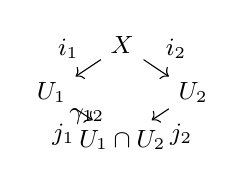
\begin{tikzpicture}[scale=0.6, every node/.style={font=\small}]
\node (X) at (0,0) {$X$};
\node (U1) at (-1.5,-1) {$U_1$};
\node (U2) at (1.5,-1) {$U_2$};
\node (U12) at (0,-2) {$U_1 \cap U_2$};
\draw[->] (X) -- (U1) node[midway, above left] {$i_1$};
\draw[->] (X) -- (U2) node[midway, above right] {$i_2$};
\draw[->] (U1) -- (U12) node[midway, below left] {$j_1$};
\draw[->] (U2) -- (U12) node[midway, below right] {$j_2$};
\node at (-0.75,-1.5) {$\gamma_{12}$};
\end{tikzpicture}
\caption{\raggedright Two-chart cover of $\mathcal{M}$ with cocycle $\gamma_{12}$ on overlap.}
\label{fig:sheaf_cover}
\end{figure}

\section{RSVP Gr\"uneisen Parameter Derivation}
\FloatBarrier
Action $\mathcal{A}[\Phi,\mathcal{v},\mathcal{S}_q] = \int \left( \frac{1}{2}(\nabla \Phi)^2 + \frac{1}{2}\|\mathcal{v}\|^2 + \lambda S_q \right) d\mu$; $\Xi = \frac{\delta \mathcal{A}}{\delta g}$; $\Gamma_{RSVP}(q) = - \frac{\partial \Xi / \partial T}{\partial^2 \mathcal{A} / \partial T^2}$ \cite{Soares2023prb,Soares2024}. At $q^*$, $\text{Curv}(\mathcal{S}_{q^*}) < \infty \implies \Gamma_{RSVP}(q^*) < \infty$ \cite{Soares2024}.

\section{Mapping Hardware to Type Systems}
\FloatBarrier
\subsection{NAND to Dependent Types Mapping}
\begin{table}[h!]
\centering
\renewcommand{\arraystretch}{1.2}
\begin{tabular}{@{}lcc@{}}
\toprule
Hardware & Boolean & Type-theoretic \\
\midrule
NAND & $\neg(A \wedge B)$ & Dependent negation of product type \cite{Girard1987} \\
AND & $A \wedge B$ & Product type $A \times B$ \cite{Girard1987} \\
OR & $A \vee B$ & Sum type $A + B$ \cite{Girard1987} \\
XOR & $A \oplus B$ & Conditional sum type \cite{Girard1987} \\
MUX & select & Pattern matching \cite{Wadler1992} \\
\bottomrule
\end{tabular}
\caption{\raggedright Mapping hardware to type systems.}
\label{tab:hardware_types}
\end{table}

\subsection{Pipelines and Compositionality}
Multi-bit buses map to vectors/indexed types, ALU to function composition, control flow to monadic sequencing/sum-type branching \cite{Coquand1988,Wadler1992}.

\section{Mechanistic Functorial Model of AI Self-Awareness}
\FloatBarrier
Categories: $\mathbf{M}$ (machine states, transitions); $\mathbf{W}$ (outcomes, belief updates). Functor $F: \mathbf{M} \to \mathbf{W}$ assigns inferred consequences \cite{Spivak2014}. Self-awareness as fixed-point $S: M \to M$, $S(M) = M \sqcup \text{ModelOf}(M)$ \cite{Bennett2025}. Mirrors RSVP: overlaps $\to$ covers; consistency $\to$ exactness; twist $\to$ adjustments \cite{MacLane1992,Awodey2010}.

\begin{figure}[H]
\centering
\begin{tikzcd}[scale=0.6, row sep=large, column sep=large, every node/.style={font=\small}]
M \arrow[r, "F"] \arrow[d, "S"'] & W \arrow[d, "\text{update}"] \\
M \sqcup \text{ModelOf}(M) \arrow[r, "F'"] & W'
\end{tikzcd}
\caption{\raggedright Functorial mapping of machine states $\mathbf{M}$ to belief updates $\mathbf{W}$ with self-awareness modeled as a fixed-point $S$.}
\label{fig:mechanistic-functor}
\end{figure}

\section{Conceptual and Mathematical Connections Between RSVP, Mechanistic AI, and Proofreading Self-Assembly}
\FloatBarrier
\subsection{Overview}
This appendix synthesizes:
1. RSVP Theory: Structured fields $(\Phi, \mathcal{v}, \mathcal{S}_q)$ with categorical and sheaf-theoretic constraints \cite{Soares2024}.
2. Mechanistic AI: Functorial operations $F$ mapping self-modeling and causal inference to field updates \cite{Bennett2025}.
3. Magnetic Proofreading Self-Assembly: Local error correction to achieve high-fidelity structures \cite{Liang2025}.
The unifying concept is local operations enforcing global constraints in entropy (RSVP), identity modeling (AI), or correct assembly (proofreading).

\subsection{RSVP Field Analogy}
Local patches $U_i \subseteq \mathcal{M}$ with fields $(\Phi|_{U_i}, \mathcal{v}|_{U_i}, \mathcal{S}_q|_{U_i})$.
- Local Entropy: $S_q(U_i) = k \frac{1 - \sum_{x \in U_i} \rho(x)^q}{q-1}$ \cite{Tsallis1988}.
- Gluing: $S_q(U_i \cup U_j) = S_q(U_i) + S_q(U_j) - S_q(U_{ij})$ \cite{MacLane1992].

\subsection{Mechanistic Functor Mapping}
Functor $F_\text{mech} \equiv F: \mathbf{Mech} \to \mathbf{RSVP}$:
\[
F(O) = (\Phi_O, \mathcal{v}_O, \mathcal{S}_O), \quad F(f: O_1 \to O_2) = (\Phi_f, \mathcal{v}_f, \mathcal{S}_f)
\]
Objects $O$ are mechanistic entities; morphisms $f$ are operations (observe, predict, act). Functoriality:
\[
F(g \circ f) = F(g) \circ F(f), \quad F(\text{id}_O) = \text{id}_{F(O)}
\]

\subsection{Proofreading Operator as Selective Entropy Update}
Inspired by Liang et al.’s magnetic decoupling \cite{Liang2025}:
1. Projector: $\Pi_\text{valid}(U_i) = \left\{ x \in U_i \mid S_q(x) \le S_\text{threshold} \right\}$.
2. Update: $F_\text{proof} : (\Phi, \mathcal{v}, \mathcal{S}_q)_{U_i} \mapsto (\Phi, \mathcal{v}, \mathcal{S}_q')_{U_i}$, where:
\[
\mathcal{S}_q'(x) = \begin{cases} S_q(x), & x \in \Pi_\text{valid}(U_i) \\ S_q(x) - \Delta S, & x \notin \Pi_\text{valid}(U_i) \end{cases}
\]
3. Gluing: $S_q(U_i \cup U_j) = S_q'(U_i) + S_q'(U_j) - S_q'(U_{ij})$.

\subsection{Summary of Analogies}
\begin{table}[h!]
\centering
\renewcommand{\arraystretch}{1.2}
\begin{tabular}{@{}lccc@{}}
\toprule
Concept & RSVP & Mechanistic AI & Magnetic Proofreading \\
\midrule
Local patch & $U_i$ & Mechanistic object $O$ & Partially assembled structure \\
Field values & $(\Phi, \mathcal{v}, \mathcal{S}_q)|_{U_i}$ & Self-model and predicted state & Magnetic dipoles / forces \\
Corrective operation & Functorial update $F_\text{proof}$ & Observe $\to$ correct $\to$ act & External field decoupling \cite{Liang2025} \\
Entropy / fidelity metric & $S_q$ & Confidence in self-model & Stability of assembly \\
Global consistency & Sheaf gluing, $\check{H}^1 = 0$ & Functor preserves composition & High-yield, low-defect product \\
\bottomrule
\end{tabular}
\caption{\raggedright Analogies between RSVP, mechanistic AI, and magnetic proofreading.}
\label{tab:analogies}
\end{table}

\subsection{Implications}
RSVP unifies bounded-entropy dynamics across physics, cognition, and self-assembly \cite{Soares2024,Bennett2025,Liang2025}.

\FloatBarrier
\sloppy
\raggedright
\bibliographystyle{plain}
\bibliography{references}

\end{document}
